\chapter{数据及观测}


\section{全球前临界PKiKP观测}

自地球内核被发现以来~\citep{lehmann1936p}已经过去将近70年,正是由于在之前被认为是内核影区的
地方发现了来自内核的绕射震相,即后临界PKiKP,才证实了内核的存在。但是由于内外核界面反射系数较小,
相比与其他界面的反射震相如PcP,前临界PKiKP的振幅很微弱,一般为PcP振幅的数十分之一,PKIKP的十分
之一左右~\citep{Bolt1965},要观测到它需要很高的信噪比,这对仪器和环境的要求也就随之提高。在内核的存在被证实后的几十年,作为其存在更为直接证据的前临界PKiKP的观测都没有报道。上世纪70年代,随着
地震台阵的发展,有关前临界PKiKP的观测结果才开始出现~\citep{Engdahl1970a}。但在单道上观测前
临界PKiKP非常困难,\citep{Shearer1990}在数万道记录中也只找到两个疑似的PKiKP相位,即使在PKiKP理论到时附近存在一个大于噪声级别的振幅,也难以断定其就是PKiKP相位。

\begin{figure}[!ht]
	\hfill{}
	\subfloat[]{\centering%
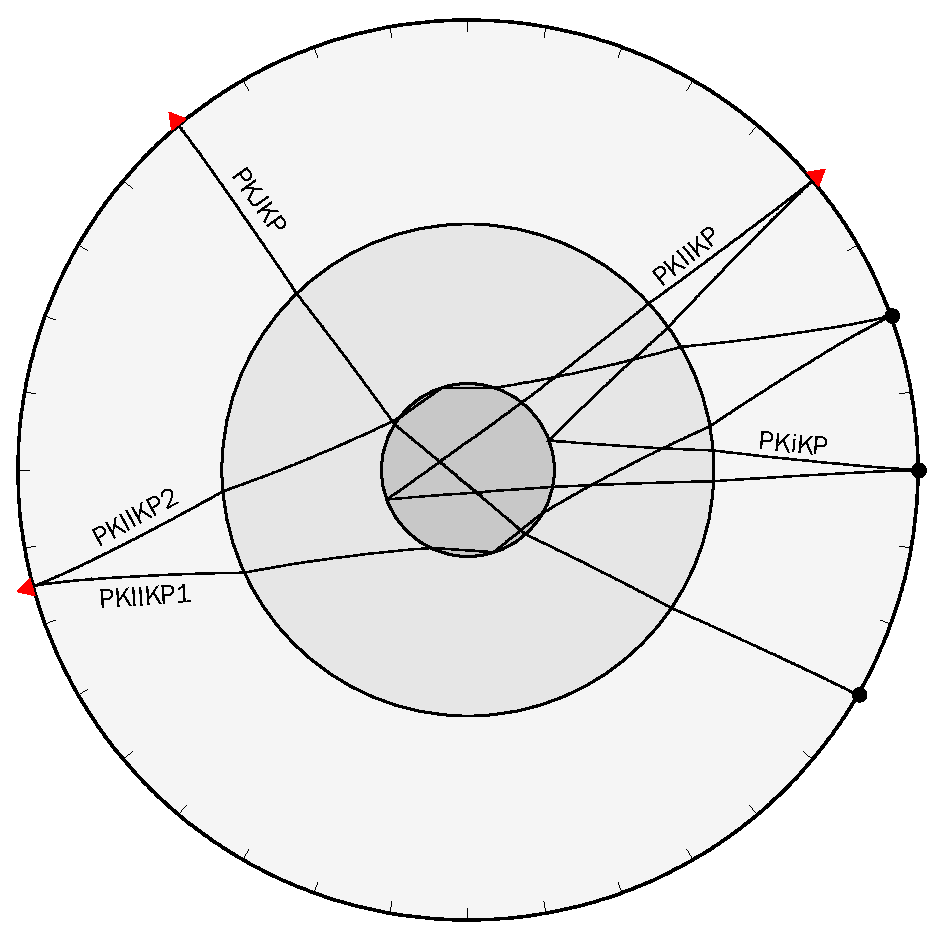
\includegraphics[width=6cm,height=6cm]{fig/chap3/path.eps}
}
	\hfill{}
	\subfloat[]{\centering%
\includegraphics[width=6cm,height=6cm]{fig/chap3/time.eps}
}
	\hfill{}
	\caption{Seismic phases which samples inner core, and their travel time %
curve.}
\end{figure}

要得到确定性的前临界PKiKP观测必须要用到台阵,而目前用来寻找前临界PKiKP的台阵又分为两种,其一是微型台阵,口径从几公里到十几公里,例如IMS台阵;其二是区域密集型台阵,口径数百公里,台站数量在几百个左右,典型的有Hi-net、USArray和阿拉斯加区域台网等。微型台阵虽然台站数量少往往在十个左右,但是能
够用于快速寻找微弱震相。因为就台阵口径而言,传播到台阵上的波已经可以看作平面波,即可以认为每个台站
接收到的是同一信号,如果在每个台站上都能看到这个相位,这就排除了特定区域的随机噪声的因素。而且当
台站间距足够小的时候,直接将所有信号直接相加就足以起到提高信噪比的作用;大口径密集台阵的优势在于, 台阵的数量还有其震中距的跨度,即增大了发现某一地震产生的前临界PKiKP相位的概率,如果台站足够多,
则能得到足够数量的PKiKP观测,再通过慢度分析就可以确定信号的来源。

最早使用微型台阵寻找前临界PKiKP的是~\cite{Souriau1989},利用WRA台阵并运用叠加方法观测到了PKiKP,由于年代较早,受限与仪器等因素,并没有在单道上看到清晰的、高信噪比的PKiKP相位。在十多年后,
\cite{Koper2003}利用全球的IMS微型台阵从1995至2000年间的数据,用台阵方法找到了数百对的PKiKP和PcP波形;而\cite{Kawakatsu2006}则利用Hi-net近700个台站的数据,观测到了自同一事件的清晰的前临界PKiKP,通过慢度分析和波形拟合,有力地证实了存在尖锐的ICB。值得注意的是,虽然相比于较早的研究
,更多的前临界PKiKP已经被发现和确认,但数据覆盖依然有限,可以看出,\cite{Koper2003}的研究中
PKiKP在ICB反射点的分布主要集中在环太平洋区域,欧亚大陆下方的ICB则没有覆盖,而且PKiKP虽然数量增
多,但很多来源与相邻的地震,其在ICB的采样点的并不具有均匀的分布,因此之前的研究未能给出ICB全球
范围的特征,区域的ICB特征也不能给出清晰的全球范围的动力学指示。

\subsection{Data}

本文除了用到先前研究所用到的IMS台阵的数据,还增加了中亚哈萨克斯坦、苏格兰、中欧还有北欧的IMS小台阵数据,而且澳大利亚及美国的IMS台阵也有所增加,所有IMS台阵的数据均从Iris数据中心获得,但先前研究
用到的CMAR和KSAR等台阵的数据不能获取。
所用到的台阵数据如下:澳大利亚的ASAR(2012-2013)、WRA(2010-2012)、PSAR(2012-2015);北美的BCAR、BMAR和IMAR(2013.11-2015.5),YKA(2013.7-2014.11),NVAR(1998-2014),ILAR,TXAR,PDAR;哈萨克斯坦的ABKAR,KKAR,MKAR;德国的GERES;
罗马尼亚的BURAR;苏格兰的EKB;挪威的SPB。所有的地震事件均选取5级以上,震中距从10到70度,震源
深度没有限制。所有的IMS台站数据均通过1-2Hz的滤波,所有的事件均通过手工挑选,保证数据的质量。
观测到的PKiKP的事件与台阵分布如图\ref{distibution},其中包含了每道都具有清晰的PKiKP相位的观测和需要叠加才能看到清晰PKiKP相位的观测。可以看到PKiKP的IMS台阵的震中距主要集中在20~40度之间,这也是前临界PKiKP在ICB反射系数最大的区间。

除了小口径台阵,这里还增加了部分阿拉斯加区域台网AK、USarray以及Hi-net的数据,观测到PKiKP相位
的震中距范围在10至50度之内。在之前的研究中除了在Hi-net上,很少有在其他台网上观测到PKiKP的报道,
追究其原因可能是,对于密集台站的台网,从大量的事件中寻找到某个能产生可观测到的PKiKP信号很困难,
这需要进行大量的数据挑选。如果台站数量达到数百个,几千个事件就会有数十万道数据的挑选工作量,但其中
可能仅有数十个事件产生的PKiKP震相能被清晰地观测到。由于PKiKP的振幅受到的影响包括(1)震源辐射花样;(2)PKiKP射线在ICB反射点的性质;(3)震源到台站路径所经过的结构效应,观测到清晰PKiKP相位需要
合适的条件。因此这里提供一种能快速找到大量PKiKP相位的方法,即先用IMS小口径台阵搜索出能产生清晰
观测的事件,这些事件就是符合产生可观测到的前临界PKiKP震相条件的,然后用附近的密集台阵数据针对某一事件搜寻PKiKP震相,这样能显著提高搜索的效率。这里就用这种方法,在AK和USArray上找到了数十道清晰的
PKiKP相位,震中距的跨度甚至能超过20度,这些是之前的研究从未观测到的结果,关于它们的情况,后面会再次提到。

\begin{figure}
	\centering
	\subfloat[]{%
\includegraphics[width=12cm,height=6cm]{fig/chap3/global.eps}
}
\\
	\subfloat[]{%
\includegraphics[width=9cm,height=6cm]{fig/chap3/hist_dist.eps}	
}
	\caption{(a)观测到PKiKP的IMS小口径台阵和事件的全球分布。红色五角星表示地震,黑色三角形%
表示台阵,黑线表示射线路径的投影。(b)所有观测到PKiKP的IMS台阵数随震中距的分布直方图。}
	\label{distibution}
\end{figure}

\subsection{Observation from global IMS stations}

\newpage

\section{PKiKP Precursor}

\newpage

\section{PKiKP Coda}


到目前为止的地震学观测表明,内核并不是一个均匀的球体,PKP和PKIKP走时的观测~\citep{Creager1992}和
自由振荡的观测~\citep{Tromp1993}都支持其内部存在各向异性; 由赤道向路径的PKIKP和PKP走时观测也表明内核
存在东西半球的地震波速差异~\citep{Tanaka1997},即内核存在1-Degree尺度的不均匀性。同时内核也被认为存在
强烈的衰减,但目前的研究主要考虑的是内核粘弹性造成的真实衰减,由于内核不均匀的尺度仍不确定,散射衰减对
经过内核的体波总体衰减的贡献也不清楚。之前的研究~\citep{Vidale2000}认为PKiKP的尾波来自外层内核不均匀体
的散射,且散射体的尺度约为2km。后续区域性的~\citep{Poupinet2004}和全球范围的PKiKP尾波研究~\citep{Koper2004}均观测到了持续200s左右的PKiKP尾波,且认为尾波来自于内核的散射。

这里结合全球范围内近十年的数据,对全球范围内观测到的PKiKP尾波进行分析。PKiKP的尾波的可能来源并不唯一,除了内核成因,其也可能来自地幔和地壳的散射。之前的研究通过对比PcP,ScP和PKiKP的尾波的差异来排除尾波地幔成因~\citep{Koper2004},然而即使是小震中距,PcP和PKiKP的路径在地幔中仍有较大的差异,尤其是在下地幔附近,因此为了确定尾波的来源还需要其他区的参照。下面采用的方法是
(1)同一事件不同区域台阵接收到的信号;(2)同一个台阵的PcP,ScP和PKiKP尾波的比较;(3)台阵接收到的发生在同一区域的不同地震的PKiKP波形的比较。

\subsection{Northern America}

2014/06/23 在ALEUTIAN群岛的事件(51.95N 178.58E,Depth 106,MB 6.0),产生的PKiKP相位
同时被位于北美的BCAR,IMAR,BMAR,YKA,NVAR和PDAR等多个IMS台阵接收到,PKiKP采样
位于阿拉斯加附近下方的ICB。图\ref{alas}显示了地震与IMS台阵的位置,以及PKiKP内核反射点的投影。

\begin{figure}[!ht]
	\centering
	\includegraphics[height=6cm,width=10cm]{fig/chap3/ALAS.eps}
	\caption{2014/06/23 22:29:51发生在ALEUTIAN群岛的事件(51.95N 178.58E,Depth 106,MB%  
6.0)和IMS台阵的位置。黑色三角形表示IMS台阵ILAR,BCAR,IMAR,BMAR,YKA,NVAR和PDAR,红色五角星表示地震位置,圆圈表示在ICB反射点的投影,其中绿色表示观测到有PKiKP,黄色表示未观测到PKiKP的台阵ILAR对应的反射点。}
	\label{alas}
\end{figure}

分别对NVAR台阵每道数据进行1-2HZ和2-3HZ频带范围的滤波,可以看出PKiKP的尾波和PKiKP主相位的能量均集中在
1-2HZ内,在2-3HZ范围内滤波后PKiKP被滤掉,每道的振幅为1-2HZ数十分之一(图\ref{nvar_sec}),且紧随着
PKiKP后面的尾波部分的振幅接近前后的噪声级别。在1175s左右似乎存在一个突然出现的能量,而且在提高滤波频率后,
振幅变得更加清晰,这是否是某个特殊的相位还有待确认。

\begin{figure}
\hfill{}
\subfloat[1-2HZ]{%
\centering
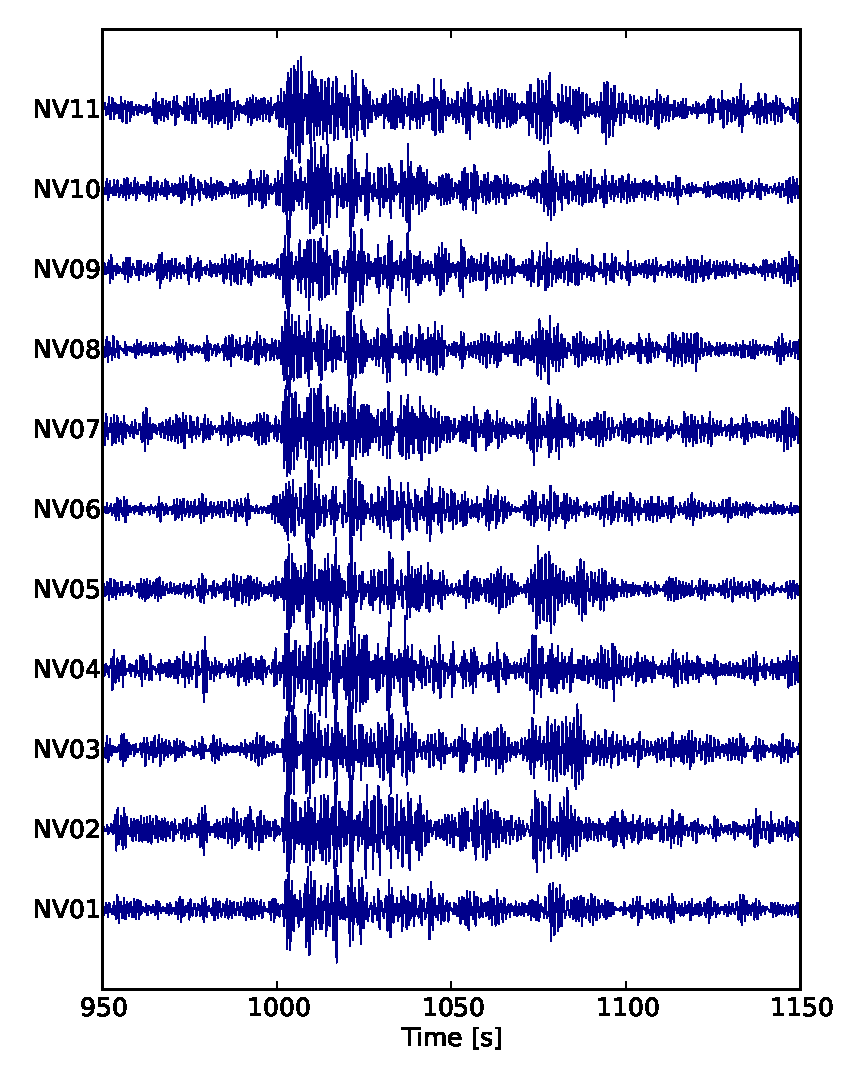
\includegraphics[width=6.5cm,height=8.5cm]{fig/chap3/nvar_sec1.eps}
}
\hfill{}
\subfloat[2-3HZ]{%
\centering
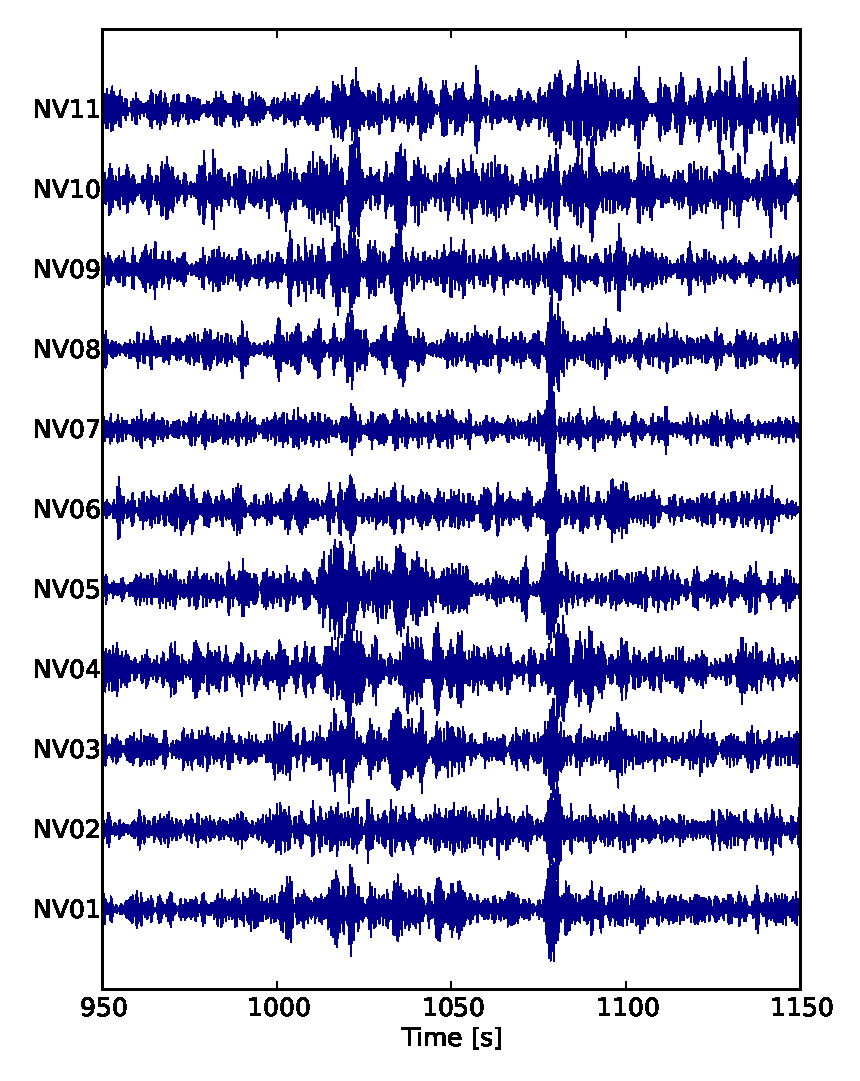
\includegraphics[width=6.5cm,height=8.5cm]{fig/chap3/nvar_sec2.eps}
}
\hfill{}
\caption{NVAR台阵记录的ALEUTIAN群岛事件的PKiKP尾波(a)经过1-2HZ滤波的结果(b)经过2-3HZ滤波的结果。}
\label{nvar_sec}
\end{figure}


与之前的研究不同,对于这个事件,NVAR台阵上观测到的PKiKP尾波的持续时间不到100s,而且在PKiKP后续50s内,
存在连续的峰值,振幅可以与PKiKP主相位相当。对PcP,ScP和PKiKP分别进行波包叠加的结果如图\ref{nvar_env},可以看出三者的尾波形态存在明显的差异。PcP的尾波在PcP最大振幅后直接衰减,ScP和PKiKP在主相位后立刻出现一个很大的振幅,但其后ScP尾波逐渐衰减到噪声级别,而PKiKP尾波振幅仍然持续到后80s左右。这说明,PKiKP的尾波与PcP和ScP的可能来源于不同的深部结构。

\begin{figure}
	\centering
	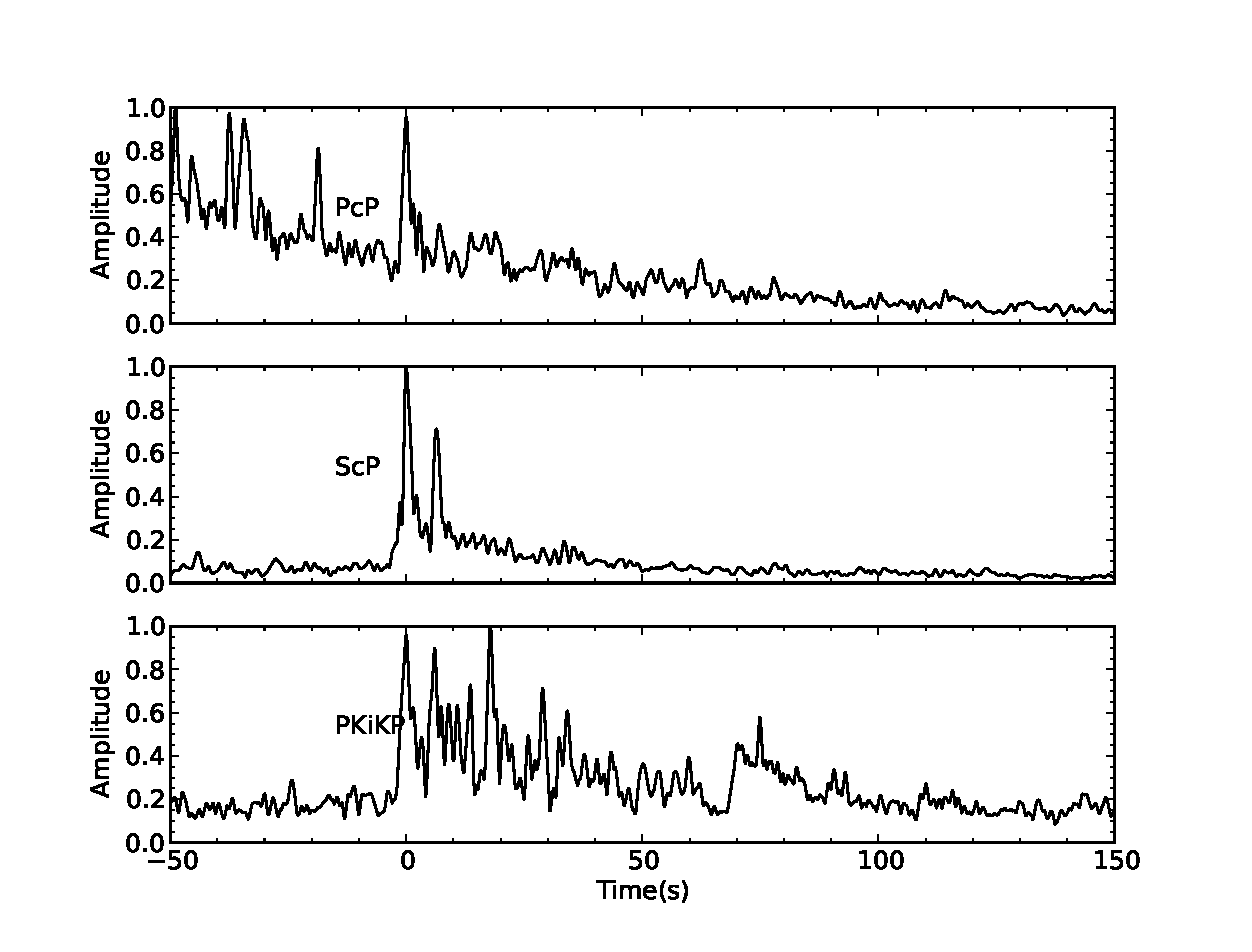
\includegraphics[width=10cm,height=7cm]{fig/chap3/nvar_env.eps}
	\caption{PcP,ScP,PKiKP的尾波波包对比,每道均按照理论的慢度进行叠加,最后再按主相位最大波包振幅%
归一化。}
	\label{nvar_env}
\end{figure}

在这些能观测到清晰PKiKP相位的IMS台阵中,只有在NVAR发现了明显的尾波,且尾波紧随PKiKP主相位,其线性叠加
和PWS叠加的结果见图\ref{nvar_mul};其他台阵上均没有发现类似的现象,PKiKP均较为清晰,且没有续至相位,
见图\ref{others},这很大程度上排除了后续的尾波来自于震源一侧,例如在震源侧反射的深度相位
;对于没有观测到PKiKP相位的台阵ILAR,在PKiKP理论到时后也没有大于噪声级别的振幅。在叠加
的PDAR台阵的PKiKP波形中,大约在主PKiKP相位后5s出现一个续至相位的振幅,这与叠加的NVAR台阵波形一致。由于
PDAR和NVAR相距较近,且相对与事件的震中距都在45\textdegree左右,这个相位可能是来源与地壳,但NVAR后续
的应该来自于更深的地方。在震中距为60\textdegree的TXAR台阵,既没有观测到直达的PKiKP相位也没有观测到任何
尾波存在的迹象。值得注意的是NVAR,PDAR和TXAR有较为接近的方位角,分别为81.4\textdegree,71.2\textdegree和79.6\textdegree。

\begin{figure}
	\centering
	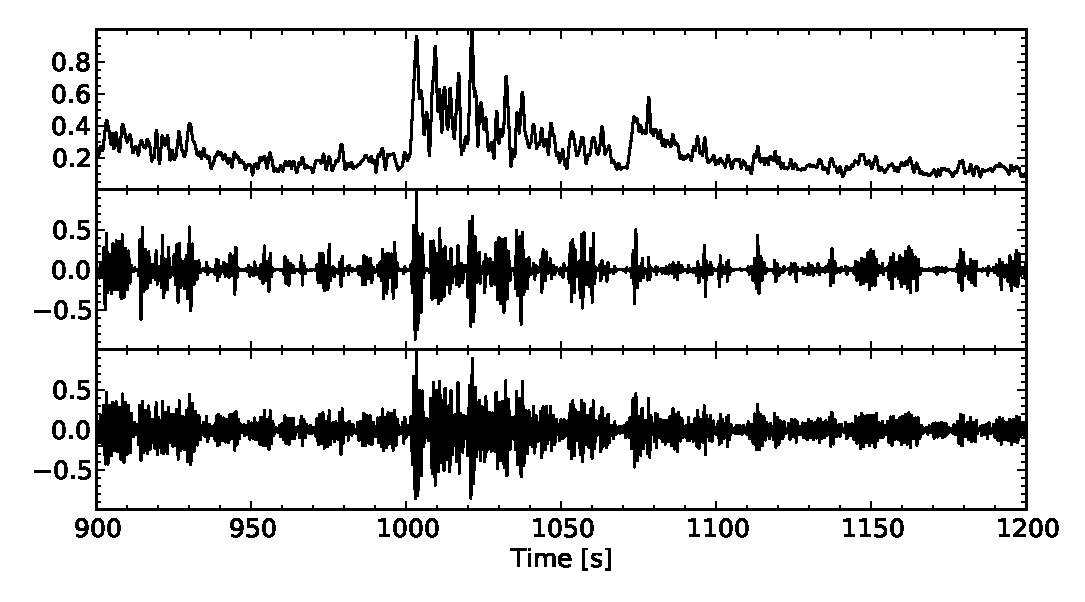
\includegraphics[width=12cm,height=6cm]{fig/chap3/nvar_mul.eps}
	\caption{NVAR台阵对2014/06/13事件的PKiKP及其尾波的叠加结果,均根据理论慢度进行叠加。上部为波包%
叠加(与图\ref{nvar_env}中的相同),中为相加权叠加(PWS),下为线性叠加,均能看到清晰的PKiKP和其后续的尾波。}
	\label{nvar_mul}
\end{figure}


\begin{figure}[tbph]
\centering
\subfloat[IMAR]{%
\centering
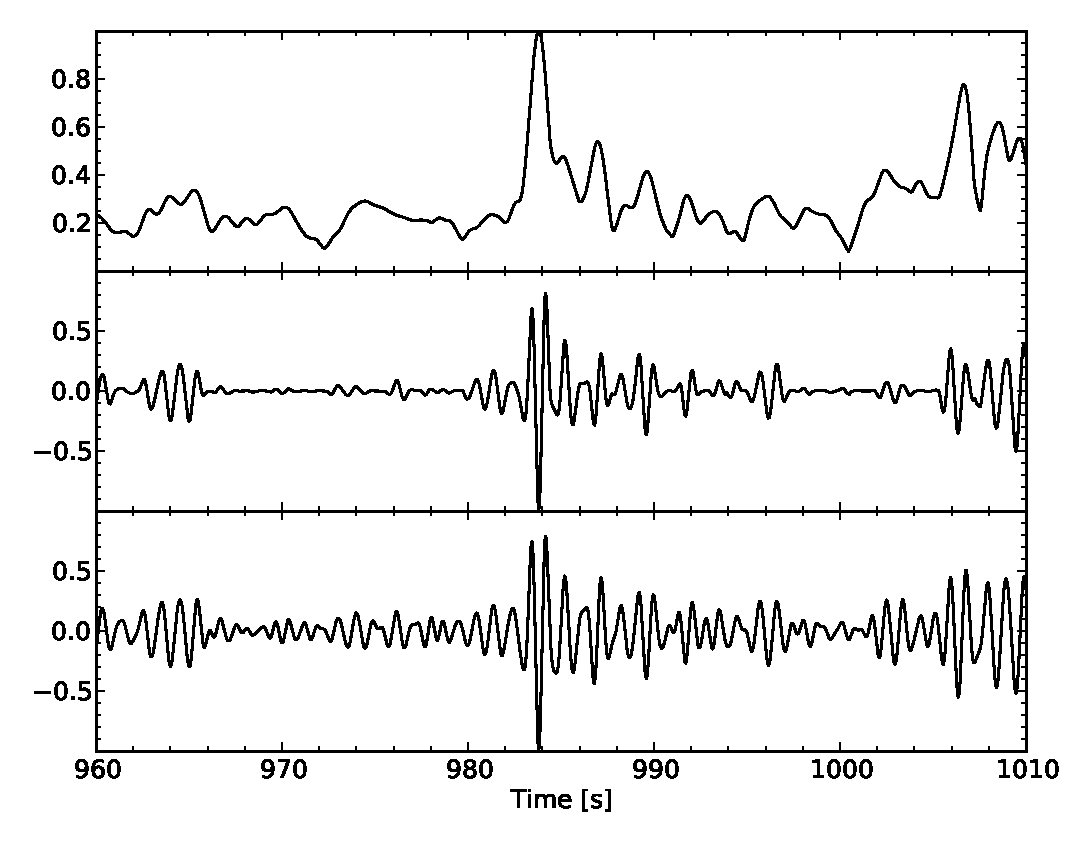
\includegraphics[width=6cm,height=4cm]{fig/chap3/imar_mul.eps}
}
\hspace{2em}
\subfloat[BCAR]{%
\centering
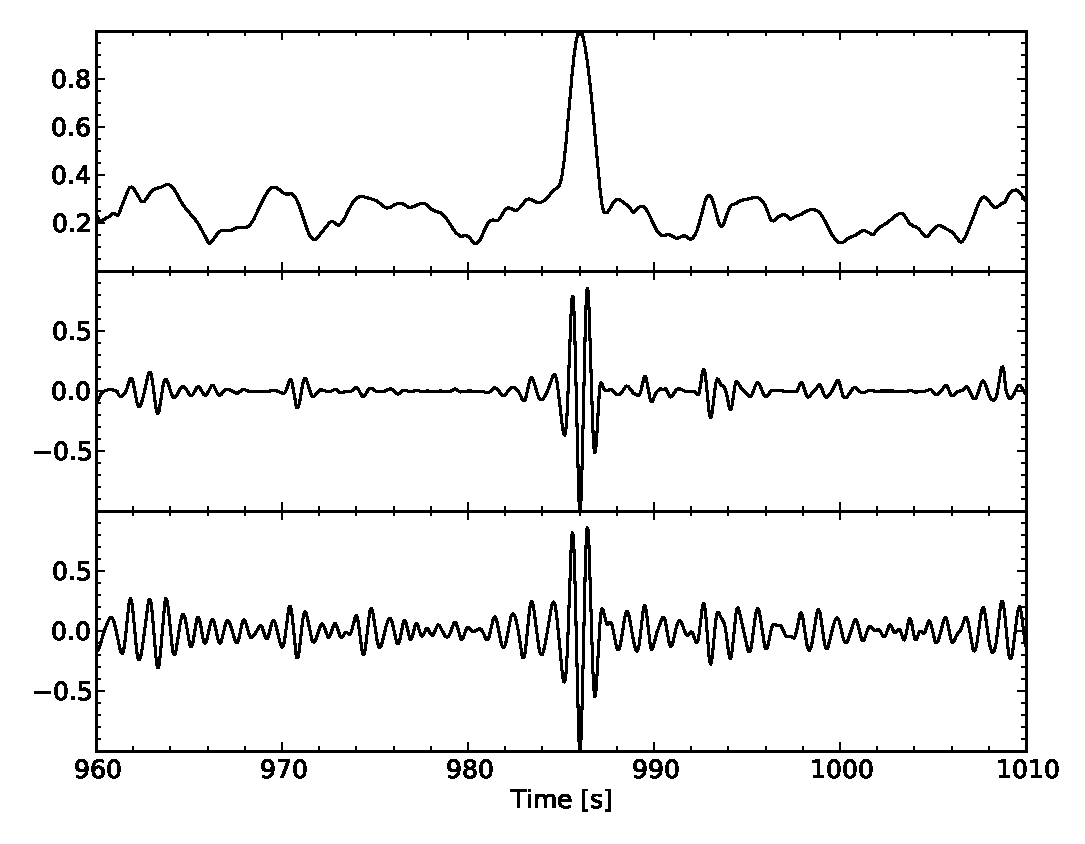
\includegraphics[width=6cm,height=4cm]{fig/chap3/bcar_mul.eps}
}\\
\subfloat[YKA]{%
\centering
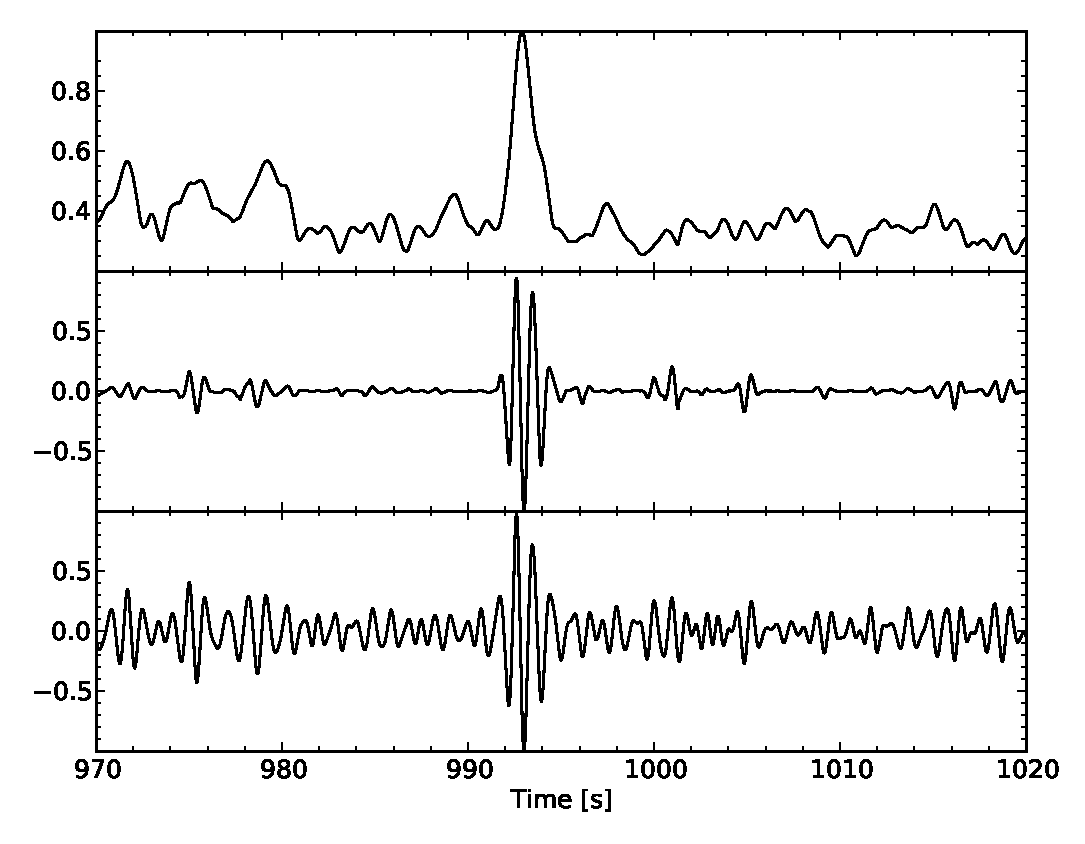
\includegraphics[width=6cm,height=4cm]{fig/chap3/yka_mul.eps}
}
\hspace{2em}
\subfloat[PDAR]{%
\centering
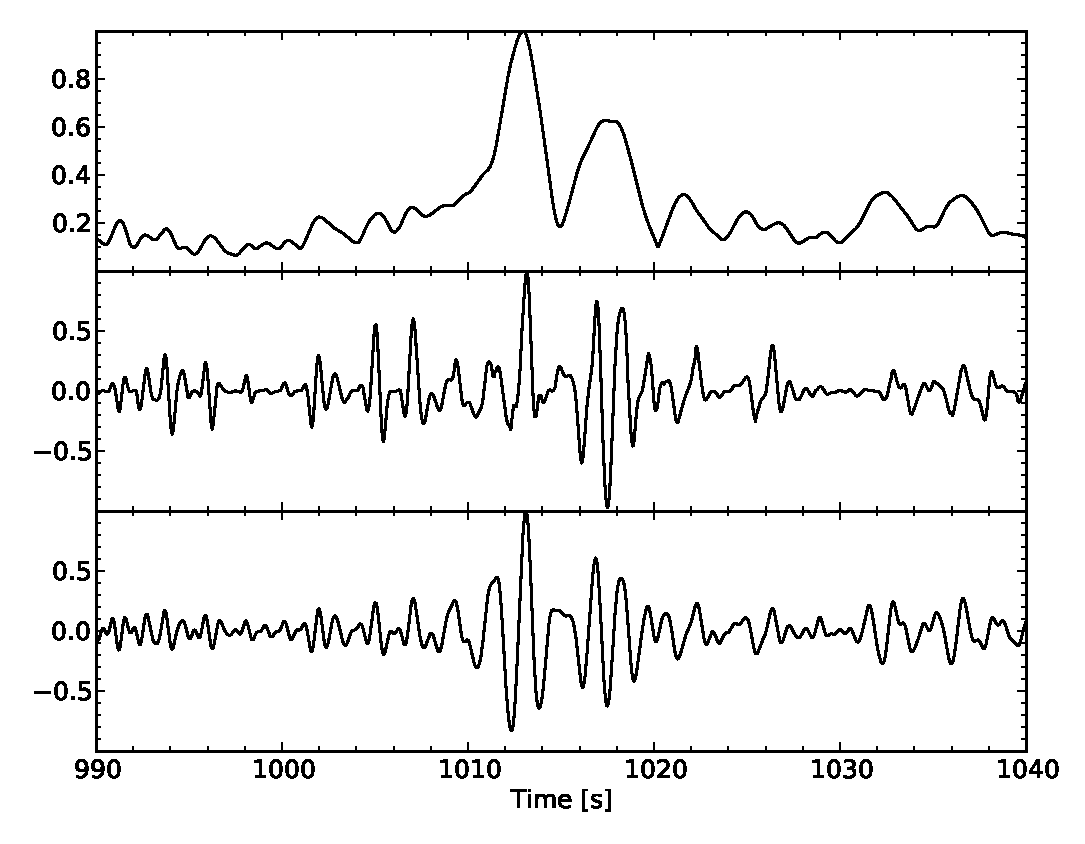
\includegraphics[width=6cm,height=4cm]{fig/chap3/pdar_mul.eps}
}
\caption{IMAR,BCAR,YKA,PDAR台阵观测到的PKiKP相位,上为波包叠加,中为PWS叠加,下为线性叠加。%
震中距分别为,19.7\textdegree,23.5\textdegree,36.0\textdegree,47.7\textdegree。}
\label{others}
\end{figure}

令人感到疑惑的是,一小时前在该事件发生处附近的另一个事件(21:11:40,51.95N 178.45E)
深度103km,震级与后者相同,但NVAR并没有记录到与该事件类似的PKiKP尾波(图\ref{nvar_mul2})。

\begin{figure}
	\centering
	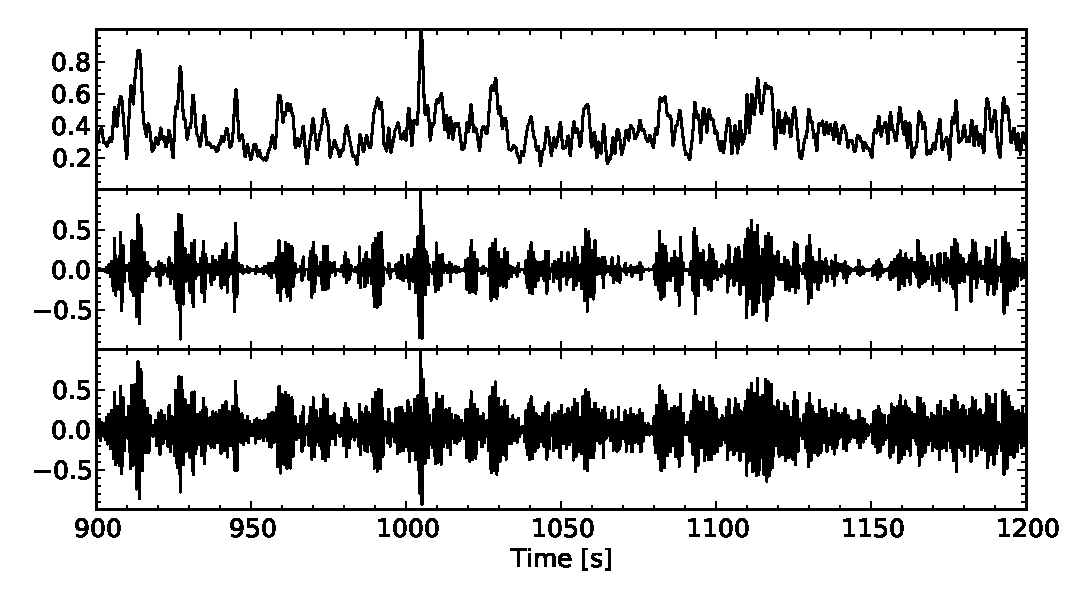
\includegraphics[width=12cm,height=6cm]{fig/chap3/nvar_mul2.eps}
	\caption{NVAR台阵对2014/06/23前一个事件的PKiKP及其尾波的叠加结果,均根据理论慢度进行叠加。%
上部为波包叠加,中为相加权叠加(PWS),下为线性叠加,可以看见明显的PKiKP,但没有明显的尾波。}
	\label{nvar_mul2}
\end{figure}

\subsection{Australia}

本文的尾波分析在澳大利亚一共用到了三个小口径台阵的数据,分别是WRA、ASAR和PSAR,它们在之前的研究中也被用到,这里增加了一个螺旋形的PSAR台阵。在这些台阵上观测到的PKiKP尾波和之前研究的有相同的特征(\ref{asar_mul}),包括长的持续时间和平滑的衰减,但并不没有之前研究所提到那么高频,进行1-2HZ的滤波后PKiKP的尾波已经具有足够大的能量,但当滤波频率提高到2-3HZ,尾波振幅则大大减小,所以1-2HZ是比较适合观测这个区域尾波的频率范围。观测到尾波的事件位置如图\ref{au_coda},可以发现这其中有很多地震的位置与之前研究中观测到尾波的事件处于同一区域,而这里使用的是完全不同时期的数据,这说明PKiKP尾波的观测是可靠的。

\begin{figure}
	\centering
	\includegraphics[width=10cm,height=8cm]{fig/chap3/AU_coda.eps}
	\caption{位于Australia的IMS台阵观测到尾波的事件,红色五角星表示地震,连接事件和台%
阵的黑色线表示射线路径的投影,黑色三角形表示台阵,台阵名在其旁边的方框中标出。}
	\label{au_coda}
\end{figure}

\begin{figure}
	\centering
	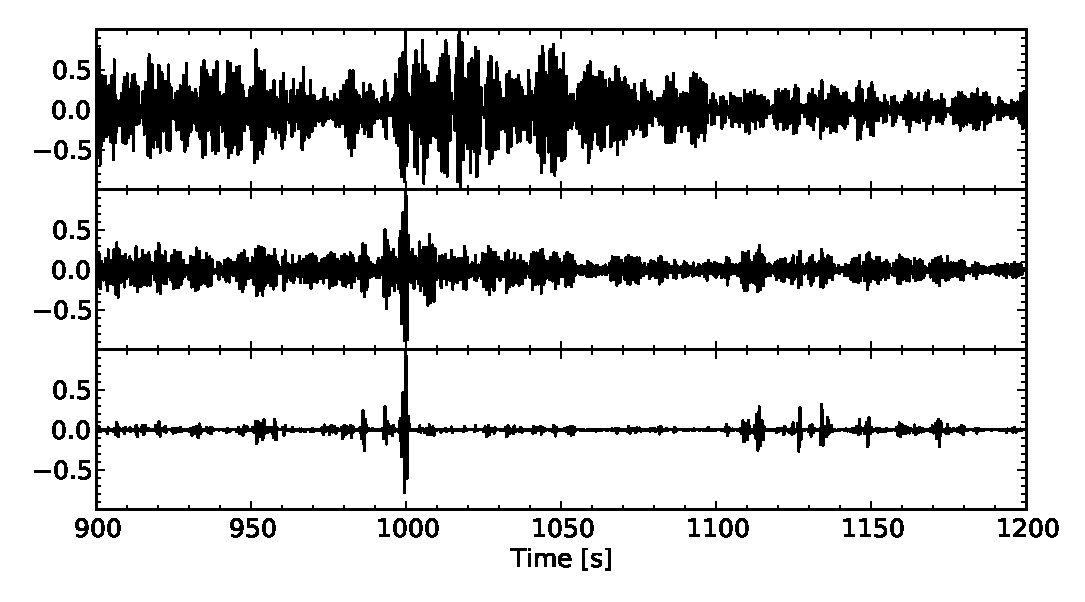
\includegraphics[width=12cm,height=6cm]{fig/chap3/asar_mul.eps}
	\caption{ASAR台阵对表中事件的PKiKP波形及其叠加结果,均根据理论慢度进行叠加。%
上部为单道波形,下为相加权叠加(PWS),中为线性叠加,可以在单道上看到很大的PKiKP尾波能量。}
	\label{asar_mul}
\end{figure}

为了确认PKiKP之后的信号确实是尾波,而非单个事件在某个台阵的产生的偶然结果,这里将ASAR台阵接收到的4个地震
事件的PKiKP附近的波形进行比较,发现均出现相似的尾波,这4个地震位置相差不到1度,且震源深度也很接近,
见表\ref{evtlst1}。由此可以推测,这可能是来自深部同一源产生的散射能量。同时可以发现,第四个事件产生的PKiKP尾波振幅较小,可能是其震级较前三个事件小(MW 5.7),激发的散射能量更小的缘故。

\begin{table}[!ht]
\centering
\begin{tabular}{*{3}{l}*{2}{c}*{2}{l}}
\hline
n & Date & Hour & Latitude & Longitude & Depth & Magnitude\\
\hline
1 & 2012/07/28 & 20:03:56.8 &  -4.651  &  153.173  &  41  & 6.5\\
2 & 2012/08/02 & 09:56:41.7 &  -4.654  &  153.275  &  46  & 6.1\\
3 & 2012/12/15 & 19:30:02.1 &  -4.632  &  153.016  &  52  & 6.1\\
4 & 2012/07/07 & 03:35:28.5 &  -4.651  &  153.296  &  35  & 5.7\\
\hline
\end{tabular}
\caption{四个位置相近的地震的震源参数。}
\label{evtlst1}
\end{table}

\begin{figure}[tbph]
	\centering
	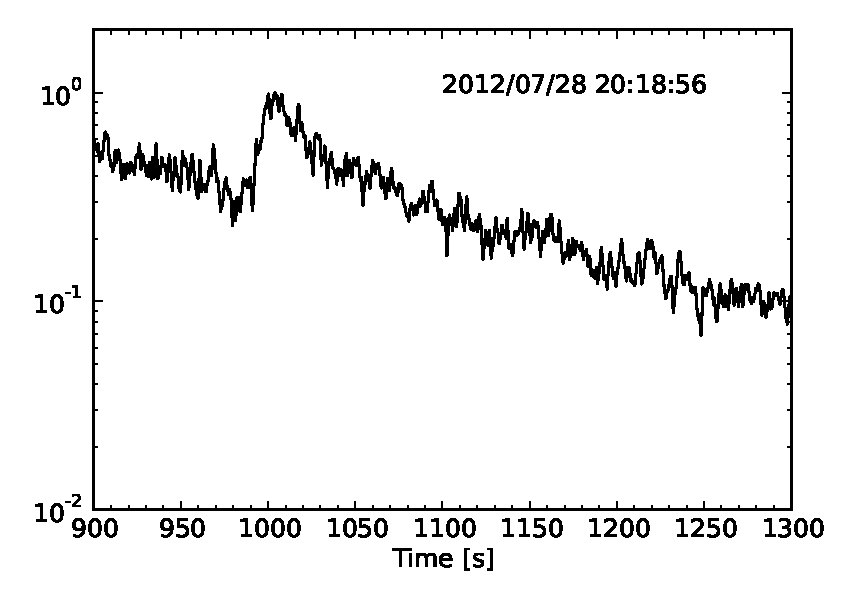
\includegraphics[width=6cm,height=4cm]{fig/chap3/3344573_coda.eps}
	\hspace{2em}
	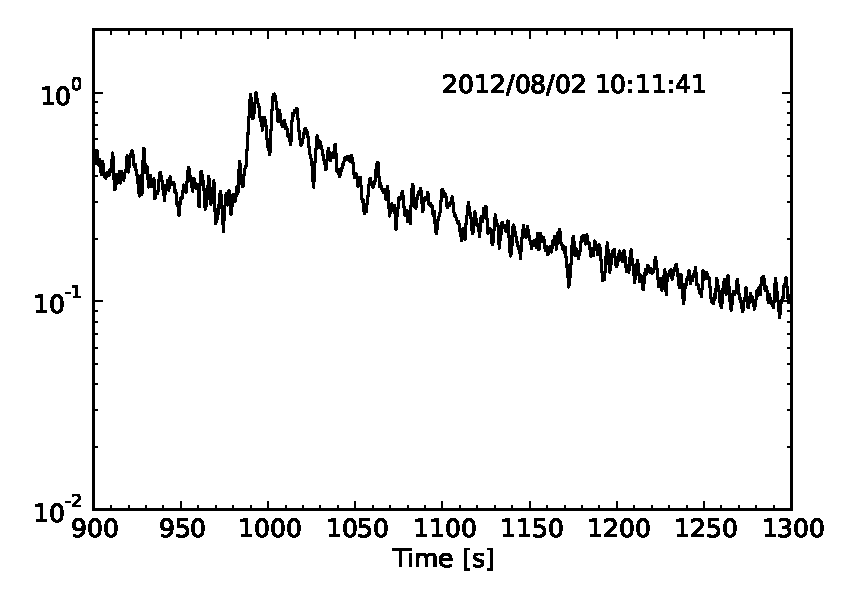
\includegraphics[width=6cm,height=4cm]{fig/chap3/3347700_coda.eps}\\
	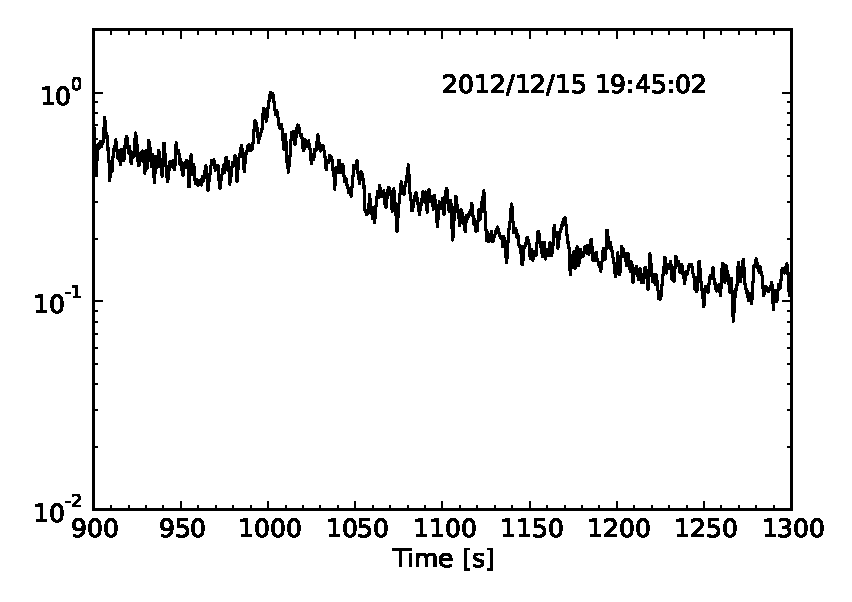
\includegraphics[width=6cm,height=4cm]{fig/chap3/3712078_coda.eps}
	\hspace{2em}
	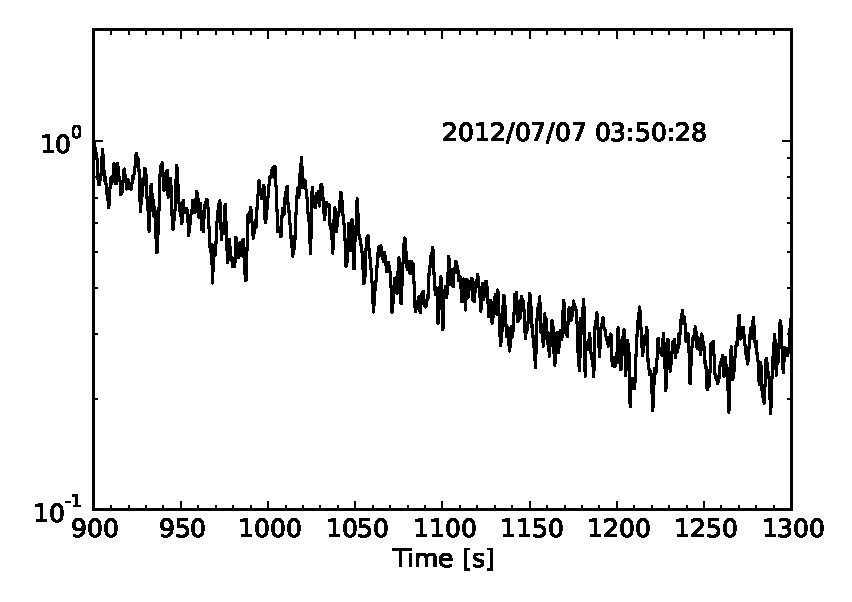
\includegraphics[width=6cm,height=4cm]{fig/chap3/3343509_coda.eps}
	\caption{4个位置接近的地震在ARSR台阵上产生的PKiKP波包叠加,频率范围为1-2HZ,它们的尾波均持续超过%
100s,图中振幅均为对数坐标。注意到第四个事件的PKiKP尾波振幅较前三个小。}
\end{figure}

之前的研究认为~\citep{Koper2004,Poupinet2004},PKiKP尾波是由之前震相的尾波,例如P,ScP的尾波与由深部散射产生的尾波叠加而成,如果拟合PKiKP到时前的波包趋势,将其向后延伸,如果其延伸之后的
曲线振幅级别小于PKiKP的尾波振幅,可以说明PKiKP之后确实有其他的能量到达台阵,其中有一部分可能是
来自内核不均匀体的散射。从ASAR台阵数据的波包叠加明显反映出这种特征。

\subsection{Asia}

位于哈萨克斯坦的IMS台阵KKAR上也观测到了PKiKP理论到时后的尾波,在记录中没有看到直达的PKiKP震
相,且从叠加的尾波波包来看,尾波大约持续100s左右,且其振幅先经历一段时期的上升,再逐渐减弱。
如图\ref{kkar_coda}。这种特征类似于~\cite{Vidale2000}的观测。

\begin{figure}[!ht]
	\centering
	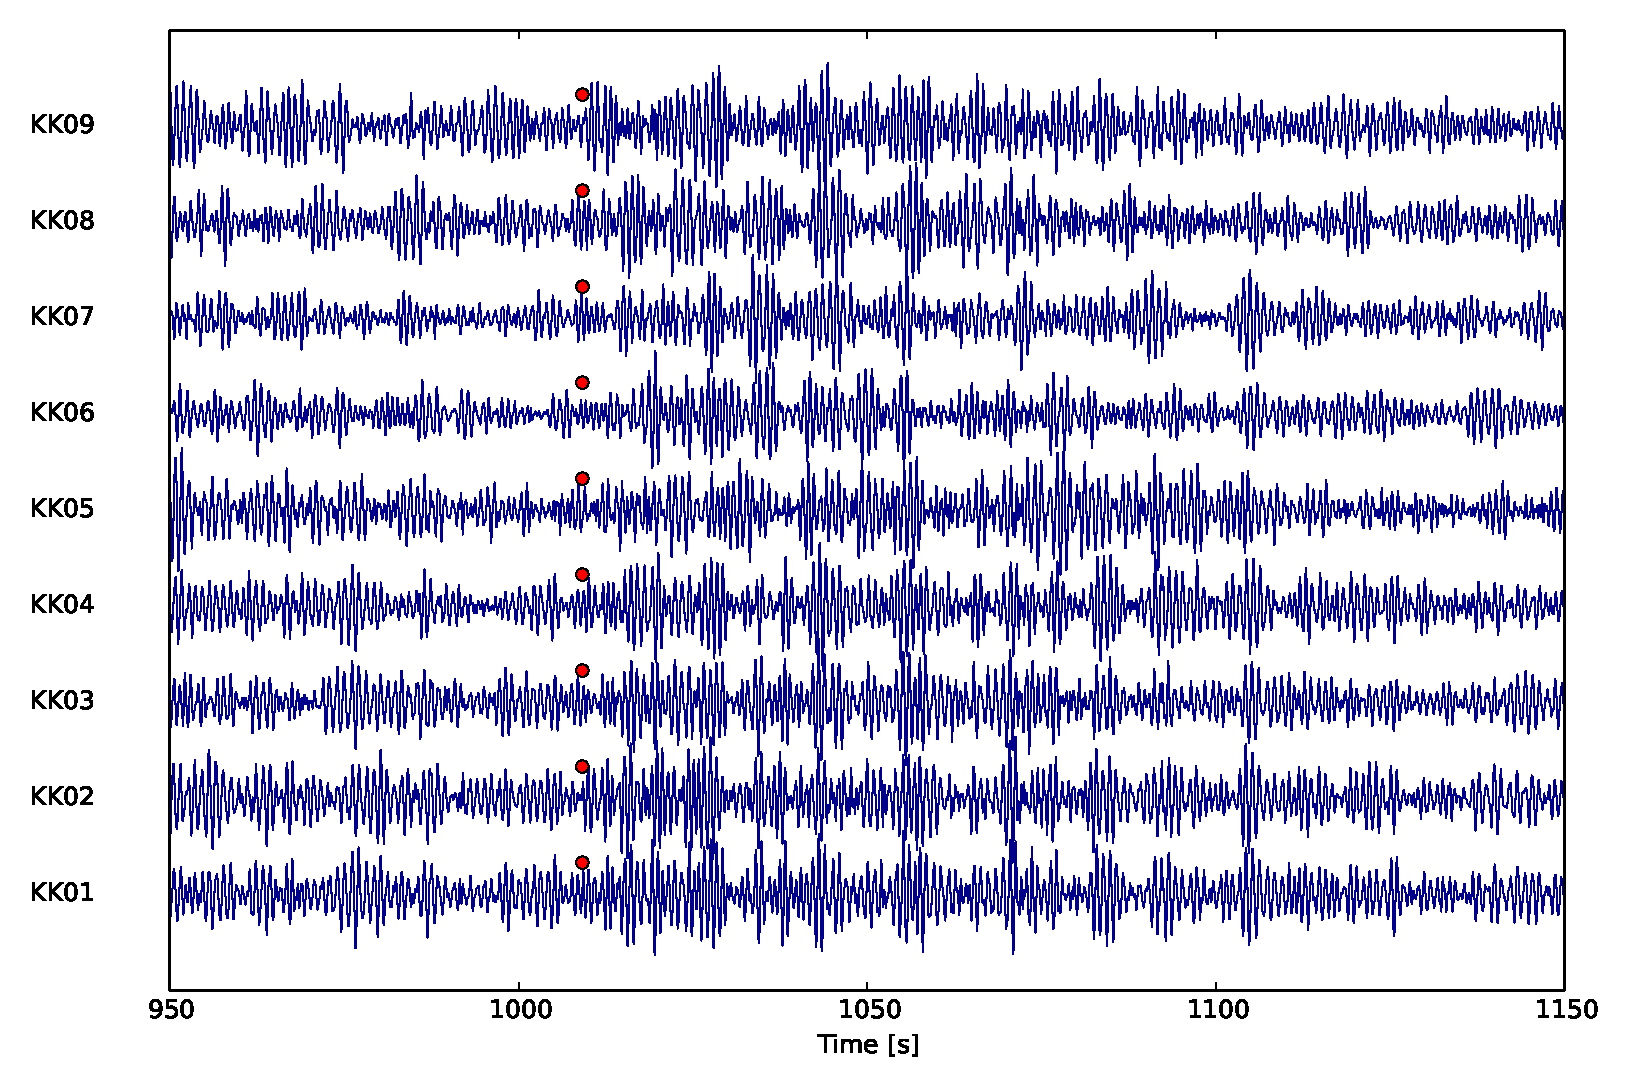
\includegraphics[width=12cm,height=6cm]{fig/chap3/kkar_sec.eps}
	\caption{KKAR台阵上观测到的尾波。红色的圆圈表示每道的PKiKP到时位置。}
	\label{kkar_coda}
\end{figure}

对于在2013年所有震中距在10{\textdegree}到70{\textdegree}的5级以上地震,这三个IMS台阵仅仅观测到这一个事件产生的明显PKiKP尾波。该事件位于位于北苏门答腊(5.42N/92.82E,depth 15.6km,MW 5.5),震中距42.4{\textdegree},ICB的反射点位于~\cite{Tanaka1997}所划定的东半球。从PWS和线性叠加的结果看来,每道PKiKP尾波并不存在明显的相关性,叠加后的振幅与前后的噪声级别
相当。

\begin{figure}[!ht]
	\centering
	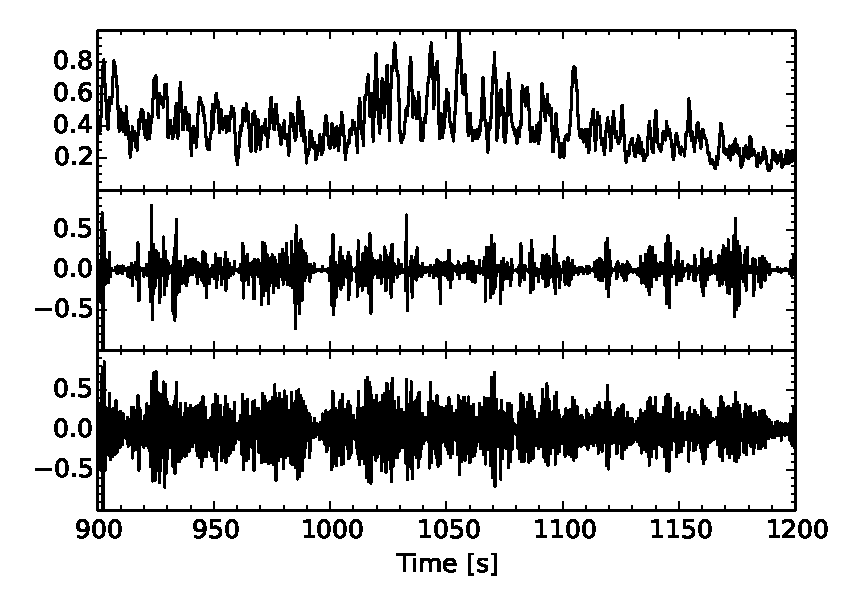
\includegraphics[width=12cm,height=6cm]{fig/chap3/kkar_mul.eps}
	\caption{KKAR台阵的PKiKP尾波叠加结果,均按照理论PKiKP慢度进行叠加。上为波包叠加,中%
间是PWS叠加,下为线性叠加。可以看到叠加的PKiKP尾波波包振幅先增大后衰减的变化。}
\end{figure}

\subsection{Conclusion about PKiKP coda observation}


